\documentclass[oneside,14pt]{extarticle}
\usepackage{cmap}
\usepackage[utf8]{inputenc}
\usepackage{longtable}
\usepackage[english,ukrainian]{babel}
\usepackage{graphicx}
\usepackage{geometry}
\usepackage{listings}
\usepackage{float}
\usepackage{amsmath}
\usepackage{subfig}
\usepackage{tempora}
\renewcommand{\arraystretch}{1.5}
\usepackage{titlesec}
\titleformat{\section}
{\centering\Large\bfseries}{\thesection}{1em}{} % Centered, large, bold font
\geometry{
	a4paper,
	left=20mm,
	right=20mm,
	top=15mm,
	bottom=15mm,
}
\lstset{
	language=c,
	tabsize=4,
	keepspaces,
	showstringspaces=false,
	frame=single,
	breaklines,
	language=C,
}
\graphicspath{ {./pictures} }
\setlength{\parindent}{4em}

\newcommand\subject{Якість програмного забезпечення та тестування}
\newcommand\lecturer{доцент кафедри ПЗ\\Фоменко А.В.}
\newcommand\teacher{асистент кафедри ПЗ\\Джумеля Е.А.}
\newcommand\mygroup{ПЗ-42}
\newcommand\lab{6}
\newcommand\theme{Пошук і документування дефектів в Jira.}
\newcommand\purpose{Протестувати свій модуль і описати знайдені дефекти і їх
	життєвий цикл в Jira}

\begin{document}
\begin{normalsize}
	\begin{titlepage}
		\thispagestyle{empty}
		\begin{center}
			\textbf{МІНІСТЕРСТВО ОСВІТИ І НАУКИ УКРАЇНИ\\
				НАЦІОНАЛЬНИЙ УНІВЕРСИТЕТ "ЛЬВІВСЬКА ПОЛІТЕХНІКА"}
		\end{center}
		\begin{flushright}
			\textbf{ІКНІ}\\
			Кафедра \textbf{ПЗ}
		\end{flushright}
		\vspace{80pt}
		\begin{center}
			\textbf{ЗВІТ}\\
			\vspace{10pt}
			до лабораторної роботи № \lab\\
			\textbf{на тему}: <<\textit{\theme}>>\\
			\textbf{з дисципліни}: <<\subject>>
		\end{center}
		\vspace{80pt}
		\begin{flushright}
			
			\textbf{Лектор}:\\
			\lecturer\\
			\vspace{28pt}
			\textbf{Виконали}:\\
			
			студенти групи \mygroup\\
			Коваленко Д.М.\\
			Снісар В.І.\\
			Баран В.Б.\\
			\vspace{28pt}
			\textbf{Прийняла}:\\
			
			\teacher\\
			
			\vspace{28pt}
			«\rule{1cm}{0.15mm}» \rule{1.5cm}{0.15mm} 2024 р.\\
			$\sum$ = \rule{1cm}{0.15mm}……………\\
			
		\end{flushright}
		\vspace{\fill}
		\begin{center}
			\textbf{Львів – 2024}
		\end{center}
	\end{titlepage}
		
	\begin{description}
		\item[Тема.] \theme.
		\item[Мета.] \purpose.
	\end{description}

    \section*{Лабораторне завдання}
    \begin{enumerate}
    	\item Обрати власний модуль з АППЗ, виділити в ньому підмодулі.
    	\item Розробити 20 і більше тестових перевірок для обраного об'єкта з
    	зазначенням модуля, що тестується і глибини тестового покриття (Smoke,
    	MAT, AT).
    	\item Сформулювати по два можливих дефекти на кожен рівень Severity
    	(Critical, Major, Average, Minor, Enhancement) для обраного об'єкта реального
    	світу.
    	\item Описати по одному дефекту на кожен рівень Severity (Critical, Major,
    	Average, Minor, Enhancement) для обраного об'єкта реального світу.
    	\item Протестувати додаток відповідно до складеної раніше тестової
    	документації.
    	\item Описати всі знайдені дефекти в звіті про дефекти в середовищі Jira.
    	\item У звіті про дефекти вказати номер збірки, яка тестується, назву
    	програми, період часу тестування, ПІБ тестувальника, тестове довкілля
    	(операційна система, браузер).
    	\item Для кожного дефекту вказати його порядовой номер, заголовок,
    	важливість, алгоритм відтворення, фактичний результат, очікуваний
    	результат, додаток, примітка.
    	\item Для кожного дефекту обов'язково зробити скріншоти.
    	\item До робочої тестової документації внести результати тестування із
    	зазначенням напроти відповідної перевірки ступеня критичності виявленого
    	дефекту, його номер і заголовок.
    	\item Оформити звіт і захистити лабораторну роботу.
    \end{enumerate}
	\section*{Хід роботи}
	
	\begin{itemize}
		\item номер збірки, що тестується – version 0.1.0;
		\item назва програми – Віртуальна лабораторія програмної інженерії (модуль проектування);
		\item тип виконуваної тестової активності - пошук і документування дефектів у Jira;
		\item період часу тестування – 210 хв;
		\item ПІБ тестувальника:
		\begin{itemize}
			\item Тестувальник 1 - Коваленко Д.М.
			\item Тестувальник 2 - Снісар В.І.
			\item Тестувальник 3 - Баран В.Б.
		\end{itemize}
		\item тестове середовище – Chromium 130.0.6723.58.
	\end{itemize}
	
	\begin{figure}[H]
		\centering
		\includegraphics[width=\columnwidth]{1}
		\caption{Повний список знайдених дефектів}
	\end{figure}
	
	\begin{figure}[H]
		\centering
		\includegraphics[width=\columnwidth]{2}
		\caption{Дефект №1}
	\end{figure}
	
	\begin{figure}[H]
		\centering
		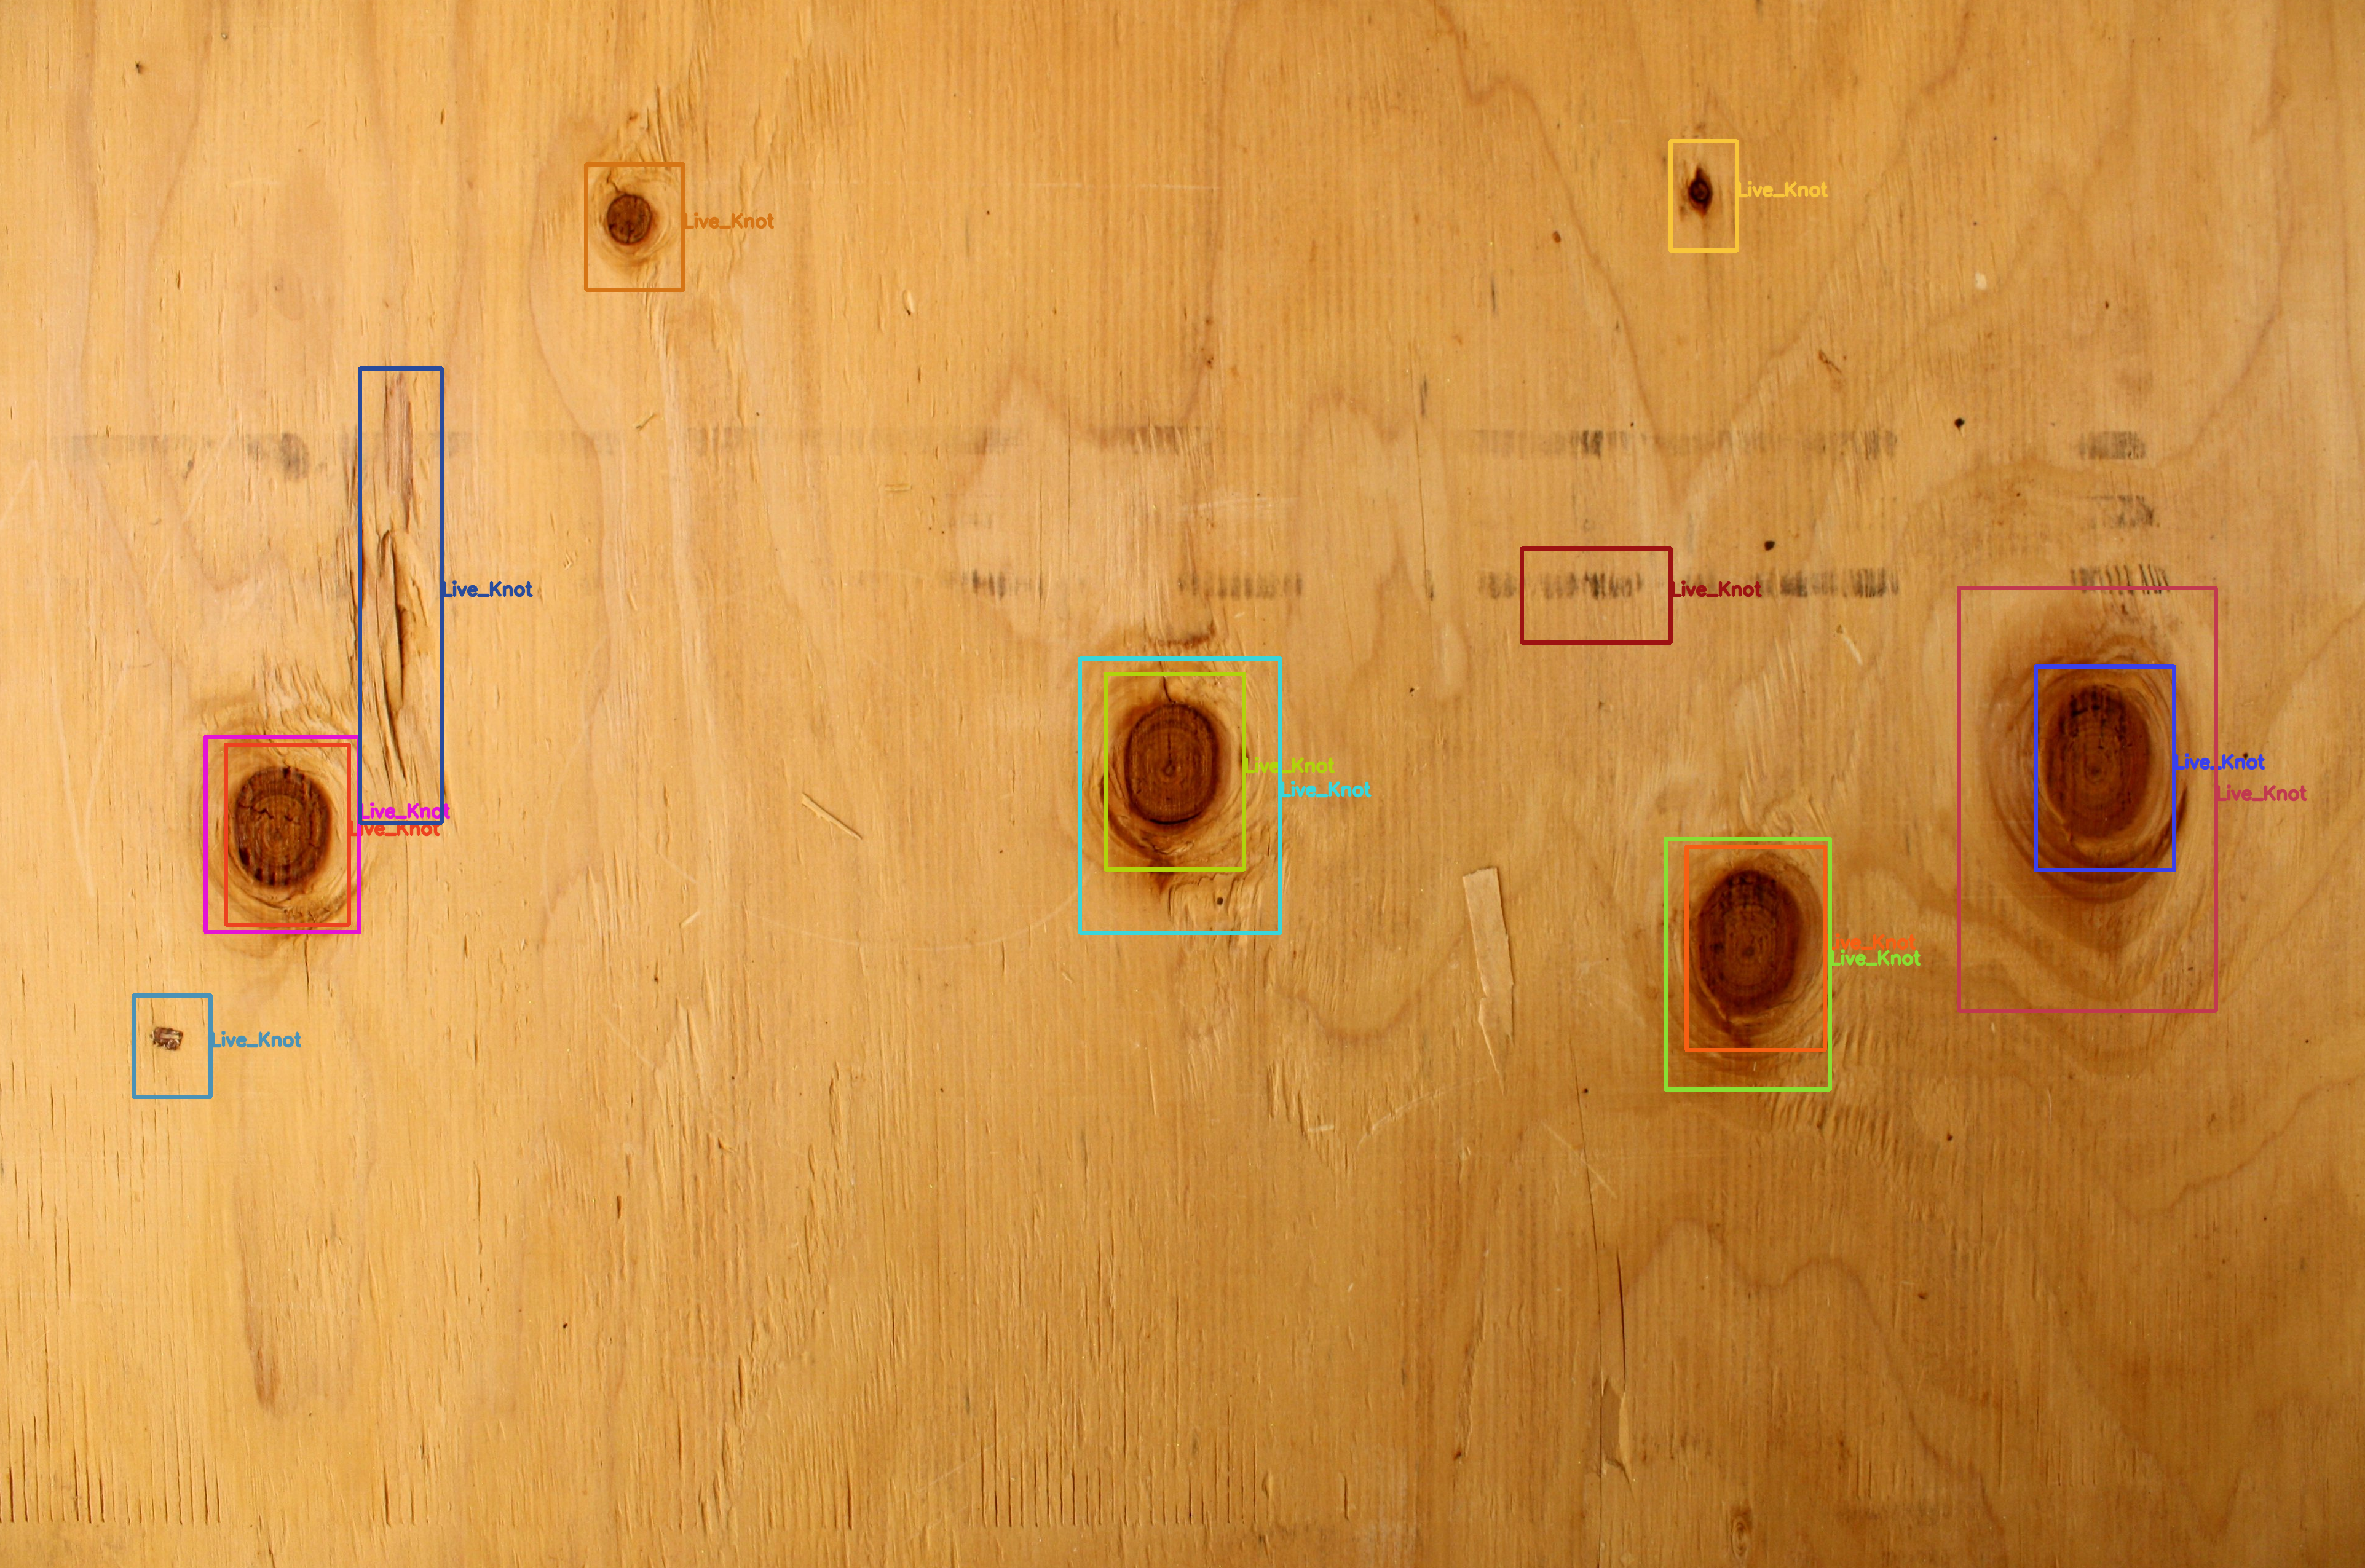
\includegraphics[width=\columnwidth]{3}
		\caption{Дефект №2}
	\end{figure}
		
	\begin{figure}[H]
		\centering
		\includegraphics[width=\columnwidth]{4}
		\caption{Дефект №3}
	\end{figure}
	
	\begin{figure}[H]
		\centering
		\includegraphics[width=\columnwidth]{5}
		\caption{Дефект №4}
	\end{figure}
	
	\begin{figure}[H]
		\centering
		\includegraphics[width=\columnwidth]{6}
		\caption{Дефект №5}
	\end{figure}
	
	\begin{figure}[H]
		\centering
		\includegraphics[width=\columnwidth]{7}
		\caption{Дефект №6}
	\end{figure}
	
	\begin{figure}[H]
		\centering
		\includegraphics[width=\columnwidth]{8}
		\caption{Дефект №7}
	\end{figure}
	
	\begin{figure}[H]
		\centering
		\includegraphics[width=\columnwidth]{9}
		\caption{Дефект №8}
	\end{figure}
	
	\begin{figure}[H]
		\centering
		\includegraphics[width=\columnwidth]{10}
		\caption{Дефект №9}
	\end{figure}
	
	\begin{figure}[H]
		\centering
		\includegraphics[width=\columnwidth]{11}
		\caption{Дефект №10}
	\end{figure}
	
	\begin{figure}[H]
		\centering
		\includegraphics[width=\columnwidth]{12}
		\caption{Дефект №11}
	\end{figure}
	
	\begin{figure}[H]
		\centering
		\includegraphics[width=\columnwidth]{13}
		\caption{Дефект №12}
	\end{figure}
	
	\begin{figure}[H]
		\centering
		\includegraphics[width=\columnwidth]{14}
		\caption{Дефект №13}
	\end{figure}
	
	\begin{figure}[H]
		\centering
		\includegraphics[width=\columnwidth]{15}
		\caption{Дефект №14}
	\end{figure}
	
	\begin{figure}[H]
		\centering
		\includegraphics[width=\columnwidth]{16}
		\caption{Дефект №15}
	\end{figure}
	
	\begin{figure}[H]
		\centering
		\includegraphics[width=\columnwidth]{17}
		\caption{Дефект №16}
	\end{figure}
	
	\begin{figure}[H]
		\centering
		\includegraphics[width=\columnwidth]{18}
		\caption{Дефект №17}
	\end{figure}
	
	\begin{figure}[H]
		\centering
		\includegraphics[width=\columnwidth]{19}
		\caption{Дефект №18}
	\end{figure}
		
	\begin{figure}[H]
		\centering
		\includegraphics[width=\columnwidth]{20}
		\caption{Дефект №19}
	\end{figure}
	
	\begin{figure}[H]
		\centering
		\includegraphics[width=\columnwidth]{21}
		\caption{Дефект №20}
	\end{figure}
	
	\begin{longtable}{|p{5cm}|p{5cm}|}
		\caption{Сценарії використання та знайдені в них дефекти}
		\\\hline
		Use case & Issues
		\\\hline
		Виконати проектну роботу & 1, 2, 5, 6, 7, 8, 9, 12, 17, 19, 20
		\\\hline
		Перевірити проектну роботу & 3, 10, 14, 16, 18
		\\\hline
		Редагувати проектну роботу & 11
		\\\hline
	\end{longtable}
	
	\begin{longtable}{|p{4cm}|p{10cm}|}
		\caption{Ступінь серйозності дефекту та відповідних йому в об’єкті реального світу (автомобіль)}
		\\\hline
		\textbf{Ступінь серйозності} & \textbf{Приклад дефекту} \\
		\hline
		Critical & Відмова гальм, що може призвести до аварії. \\
		\hline
		Major & Проблеми з трансмісією, які ускладнюють перемикання передач. \\
		\hline
		Average & Витік масла, що може призвести до зниження продуктивності двигуна. \\
		\hline
		Minor & Подряпини на кузові, які не впливають на функціональність автомобіля. \\
		\hline
		Enhancement & Встановлення нової інформаційно-розважальної системи з підтримкою Apple CarPlay. \\
		\hline
	\end{longtable}
	
	\section*{Висновки}
	ПІд час виконання лабораторної роботи розроблено 20 тестових перевірок для модуля проектування. Описано всі дефекти в середовищі Jira. Для кожного дефекту вказано його порядковий номер, заголовок, важливість, алгоритм відтворення, фактичний результат, очікуваний результат. Описано по одному дефекту на кожен рівень серйозності для обраного об'єкта реального світу.
	    
\end{normalsize}
\end{document}
